\documentclass[handouts,hyperref={pdfpagelabels=false}]{beamer}
\let\Tiny=\tiny
\usetheme{Copenhagen}
\usepackage[T1]{fontenc}
\usepackage[utf8]{inputenc}
\usepackage[greek,english]{babel}
\usepackage[fixlanguage]{babelbib}
\usepackage{hyperref}
\selectbiblanguage{greek}
\graphicspath{ {images/} }

\hypersetup{
  unicode=true,
  colorlinks=true,
  % linkcolor=green,
  citecolor=red,
  % filecolor=blue,
  urlcolor=blue,
  % pdftitle=,
  % pdfauthor=,
  % pdfsubject=,
  % pdfkeywords=
}

\begin{document}
\selectlanguage{greek}

\title{Ανίχνευση Επιθέσεων σε Ασύρματα Δίκτυα μέσω Αναγνώρισης Ανωμαλιών στη Δικτυακή Κίνηση}
\author{Δημήτριος Πολίτης}
\institute{
  Εθνικό Μετσόβιο Πολυτεχνείο\\
  Σχολή Ηλεκτρολόγων Μηχανικών και Μηχανικών Η/Υ\\
}

\begin{frame}
\titlepage
\end{frame}

\begin{frame}
\frametitle{Περίγραμμα Παρουσίασης}
\tableofcontents
\end{frame}

\section{\foreignlanguage{greek}{Εισαγωγή}}
\begin{frame}
\frametitle{\foreignlanguage{greek}{Ασφάλεια ΠΣ}}

\begin{block}{Ασφάλεια Πληροφοριακών Συστημάτων}
\begin{itemize}
  \item Τα πληροφοριακά συστήματα ενσωματώνονται στην καθημερινότητά μας
  \item Η ασφάλεια των ΠΣ γίνεται απαραίτητη
\end{itemize}
\end{block}

\begin{block}{Αποτροπή Πρόσβασης - Ανίχνευση Επιθέσεων}
\begin{itemize}
  \item Το πρώτο επίπεδο ασφάλειας είναι η αποτροπή πρόσβασης \textlatin{IPS}
  \begin{itemize}
    \item Κωδικοί πρόσβασης
    \item \textlatin{Two factor authentication}
  \end{itemize}
  \item Το δεύτερο επίπεδο είναι η ανίχνευση επιθέσεων \textlatin{IDS}
  \item Το τρίτο επίπεδο είναι η ανοχή - αντίδραση (\textlatin{responce and tolerance})
\end{itemize}
\end{block}
\end{frame}

\section{\foreignlanguage{greek}{Κίνητρο - Υπόβαθρο}}
\begin{frame}
\frametitle{\foreignlanguage{greek}{Διαφορές Ασύρματων - Ενσύρματων Δικτύων}}
\begin{block}{Διαφορές Ασύρματων - Ενσύρματων Δικτύων}
\begin{itemize}
    \item Δεν υπάρχει απομόνωση φυσικού μέσου.
    \item Δεν υπάρχει ισχυρή δικτυακή υποδομή
    \item Μεγάλη κινητικότητα κόμβων
    \item Παρεμβολές, θόρυβος, απώλειες πακέτων, θερμοκρασία, υγρασία
    \item Πληθώρα πελατών που εισέρχονται και εξέρχονται τυχαία
  \end{itemize}
Οι διαφορές στους δυο τύπους δικτύων επιβάλουν την μελέτη νέων μεθόδων ανίχνευσης επιθέσεων στα ασύρματα δίκτυα.
\end{block}
\end{frame}

\section{\foreignlanguage{greek}{Απειλές σε Ασύρματα Δίκτυα}}
\begin{frame}
\frametitle{\foreignlanguage{greek}{Τύποι Ασύρματων Δικτύων}}
\begin{block}{Τύποι Ασύρματων Δικτύων}
\begin{itemize}
    \item \textlatin{Wireless local area networks}
    \item \textlatin{Wireless personal area networks}
    \item \textlatin{Wireless sensor networks}
    \item \textlatin{Ad hoc networks}
    \item \textlatin{Mobile telephony}
    \item \textlatin{Wireless mesh networks}
    \item \textlatin{Cyber physical systems}
\end{itemize}
\end{block}
\end{frame}

\begin{frame}
\frametitle{\foreignlanguage{greek}{Απειλές Ασύρματων Δικτύων}}
\begin{itemize}
    \item \textlatin{Silencing}
    \item \textlatin{Spoofing}
    \item \textlatin{Sybil attack}
    \item \textlatin{Jamming}
    \item \textlatin{Tampering}
    \item \textlatin{Node capture}
    \item \textlatin{Sinkhole attack}
    \item \textlatin{Denial of service}
    \item \textlatin{Selective forwarding}
    \item \textlatin{Wormhole attack}
    \item \textlatin{Blackhole attack}
    \item \textlatin{Routing request flooding attack}
    \item \textlatin{Routing request disrupt attack}
    \item \textlatin{Eavesdropping}
\end{itemize}
\end{frame}

\section{\foreignlanguage{greek}{Ανίχνευση Εισβολών με Ανάλυση της κίνησης}}
\begin{frame}
\frametitle{\foreignlanguage{greek}{Συστήματα \textlatin{IDS}}}
\begin{block}{Κύριες Λειτουργίες \textlatin{IDS}}
\begin{itemize}
    \item Συλλογή δεδομένων δικτυακής κίνησης
    \item Ανάλυση δεδομένων με χρήση τεχνικών ανίχνευσης επιθέσεων
\end{itemize}
\end{block}

\begin{block}{Μετρικές Αποτελεσματικότητας \textlatin{IDS}}
\begin{itemize}
    \item \textlatin{False Positive Rate (FPR)}
    \item \textlatin{False Negative Rate (FNR)}
    \item \textlatin{Detection Rate (DR)}
\end{itemize}
Η ευαισθησία του συστήματος ανίχνευσης υπολογίζεται από τη σχέση:
\[DR = 1 - FPR - FNR\]
\end{block}
\end{frame}

\begin{frame}
\frametitle{\foreignlanguage{greek}{Συλλογή και Ανάλυση Δεδομένων}}
\begin{block}{Συλλογή Δεδομένων}
\begin{itemize}
    \item \textlatin{traffic based collection}
    \item \textlatin{behavior based collection}
\end{itemize}
\end{block}
\begin{figure}
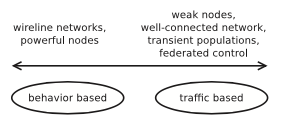
\includegraphics[scale=0.6]{coll-appr}
\caption{Διαδικασία συλλογής δεδομένων}
\end{figure}
\end{frame}

\begin{frame}
\frametitle{\foreignlanguage{greek}{Συλλογή και Ανάλυση Δεδομένων}}
\begin{block}{Ανάλυση Δεδομένων}
\begin{itemize}
    \item \textlatin{data minning}
    \item \textlatin{pattern matching}
\end{itemize}
\end{block}
\begin{figure}
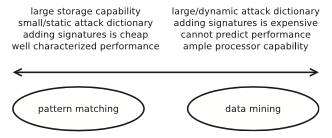
\includegraphics[scale=0.6]{anal-appr}
\caption{Διαδικασία ανάλυσης δεδομένων}
\end{figure}
\end{frame}

\begin{frame}
\frametitle{\foreignlanguage{greek}{Ανίχνευση Επιθέσεων}}
\begin{block}{Ανίχνευση Επιθέσεων}
\begin{itemize}
    \item \textlatin{anomaly based}
    \item \textlatin{specification based}
    \item \textlatin{reputation based management}
    \item \textlatin{signature based}
\end{itemize}
\end{block}
\end{frame}

\begin{frame}
\frametitle{\foreignlanguage{greek}{Τύποι Ανωμαλιών στη Δικτυακή Κίνηση}}
\begin{block}{Κύριοι Τύποι αποκλίσεων}
\begin{itemize}
    \item \textlatin{point anomalies}
    \item \textlatin{context anomalies}
    \item \textlatin{collective anomalies}
\end{itemize}
\end{block}
\end{frame}

\begin{frame}
\frametitle{\foreignlanguage{greek}{Τρόποι Λειτουργίας Τεχνικών Ανίχνευσης}}
\begin{block}{Με βάση τα δεδομένα εκπαίδευσης}
\begin{itemize}
    \item \textlatin{Supervised Methods}
    \item \textlatin{Semisupervised Methods}
    \item \textlatin{Unsupervised Methods}
\end{itemize}
\end{block}

\begin{block}{Με βάση τον αλγόριθμο ανίχνευσης}
\begin{itemize}
    \item \textlatin{Classification based (Neural Networks, Bayesian Networks, Support Vector Machines, Rule-Based)}
    \item \textlatin{Nearest Neighboor Based}
    \item \textlatin{Clustering Based}
    \item \textlatin{Statistical Based (Parametric, non-Parametric)}
    \item \textlatin{Information Theory Based}
\end{itemize}
\end{block}
\end{frame}

\begin{frame}
\frametitle{\foreignlanguage{greek}{Αποτελεσματικότητα Ανίχνευσης \textlatin{anomaly based}}}
\begin{block}{Πλεονεκτήματα}
\begin{itemize}
    \item Δεν αναζητούν κάτι συγκεκριμένο - οχι \textlatin{attack dictionaries}
    \item Μεγάλο πλήθος εφαρμογών
    \item Ενδείκνειται για ασύρματους κόμβους με μικρό αποθηκευτικό χώρο
\end{itemize}
\end{block}

\begin{block}{Μειονεκτήματα}
\begin{itemize}
    \item Yψηλό \textlatin{FPR}
    \item Δυσκολία κατά τη δημιουργία του μοντέλου και των δεδομένων εκπαίδευσης
\end{itemize}
\end{block}
\end{frame}

\begin{frame}[allowframebreaks]
\frametitle{\foreignlanguage{greek}{Βιβλιογραφία}}
\nocite{*}
\bibliographystyle{babplain}
\bibliography{cellular_net}
\end{frame}

\end{document}